\chapter[BRT]{Boosted Regression Trees}

\begin{objetivos}
By the end of this chapter, readers should understand boosted regression trees
(BRTs); fit BRT presence--background models; control hyperparameters to reduce
overfitting; select the optimal number of trees by cross-validation; evaluate
models using AUC, TSS, sensitivity, and specificity; interpret relative
predictor importance and partial response curves; map suitability for
\textit{Dinizia excelsa}; and compare BRT with GLM, GAM, and Random Forest.
\end{objetivos}

\section{Introduction}

BRT combines decision trees with boosting. Unlike Random Forest, which fits
many largely independent trees and aggregates their predictions, boosting fits
trees sequentially so that each new tree improves residual errors from the
preceding ensemble. BRTs are widely used in SDM because they represent
nonlinear responses, predictor interactions, and complex environmental patterns
\parencite{elith2008working,elith2009,guisan2017habitat}.

\begin{conceito}[title={\faBook\quad BRT in SDM}]
BRT combines decision trees with sequential learning. It can represent complex
ecological relationships but requires careful hyperparameter control to avoid
overfitting.
\end{conceito}

\section{Main Hyperparameters}

The principal BRT hyperparameters are:
\begin{itemize}
  \item \texttt{n.trees}: maximum number of trees;
  \item \texttt{interaction.depth}: interaction complexity;
  \item \texttt{shrinkage}: learning rate;
  \item \texttt{bag.fraction}: fraction of observations used in each iteration; and
  \item \texttt{n.minobsinnode}: minimum observations in terminal nodes.
\end{itemize}

\begin{atencao}[title={\faExclamationTriangle\quad BRT and overfitting}]
BRT may overfit when the number of trees is excessive, the learning rate is
inappropriate, or trees are too deep. The optimal number of trees should be
selected by cross-validation.
\end{atencao}

\section{Data Preparation}
\rscriptfile{scripts/unidade09/01_estrutura_pastas.R}
\rscriptfile{scripts/unidade09/02_preparar_dados_brt.R}

\section{Fitting the BRT}

The BRT uses a Bernoulli distribution for binary presence--background data. The
optimal number of trees is selected using internal cross-validation.

\rscriptfile{scripts/unidade09/03_ajustar_brt_dinizia.R}

\begin{figure}[H]
  \centering
  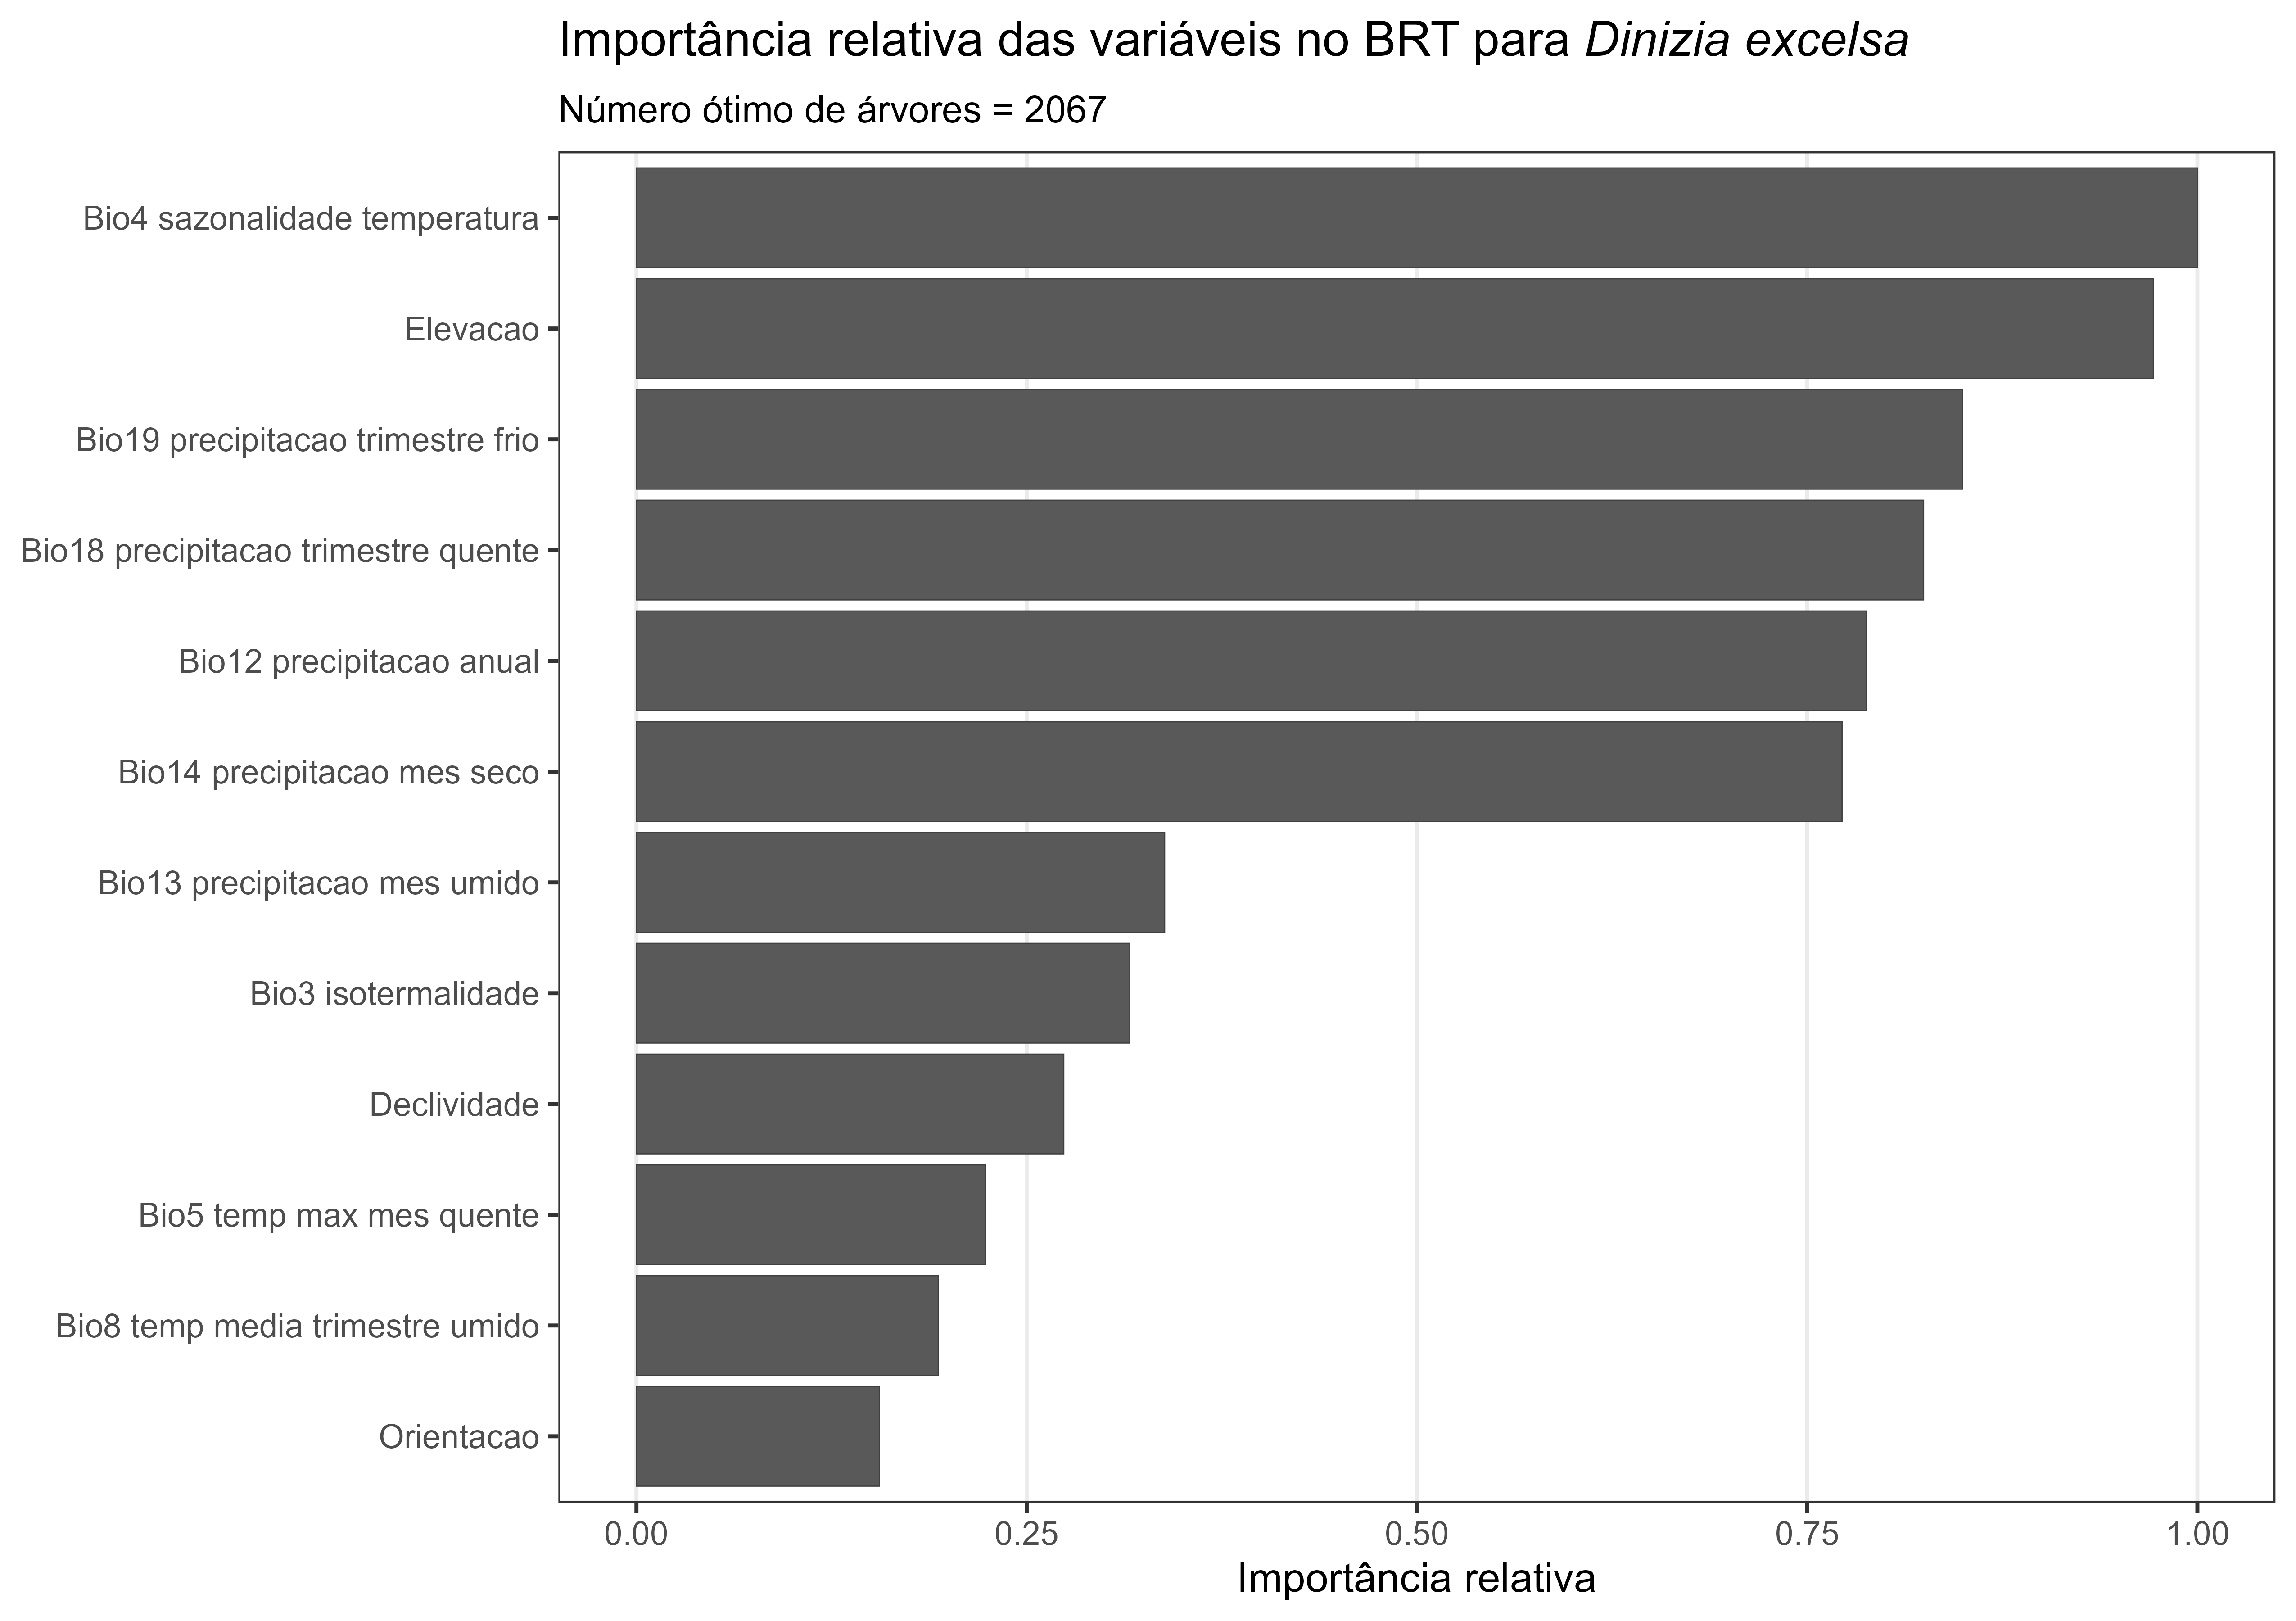
\includegraphics[width=0.86\textwidth]{figuras/unidade09/unidade09_importancia_variaveis_brt.png}
  \caption{Relative importance of environmental predictors in the BRT fitted to \textit{Dinizia excelsa}.}
  \label{fig:unidade09_importancia_brt}
\end{figure}

\section{Model Evaluation}
\rscriptfile{scripts/unidade09/04_avaliar_brt_dinizia.R}

\begin{figure}[H]
  \centering
  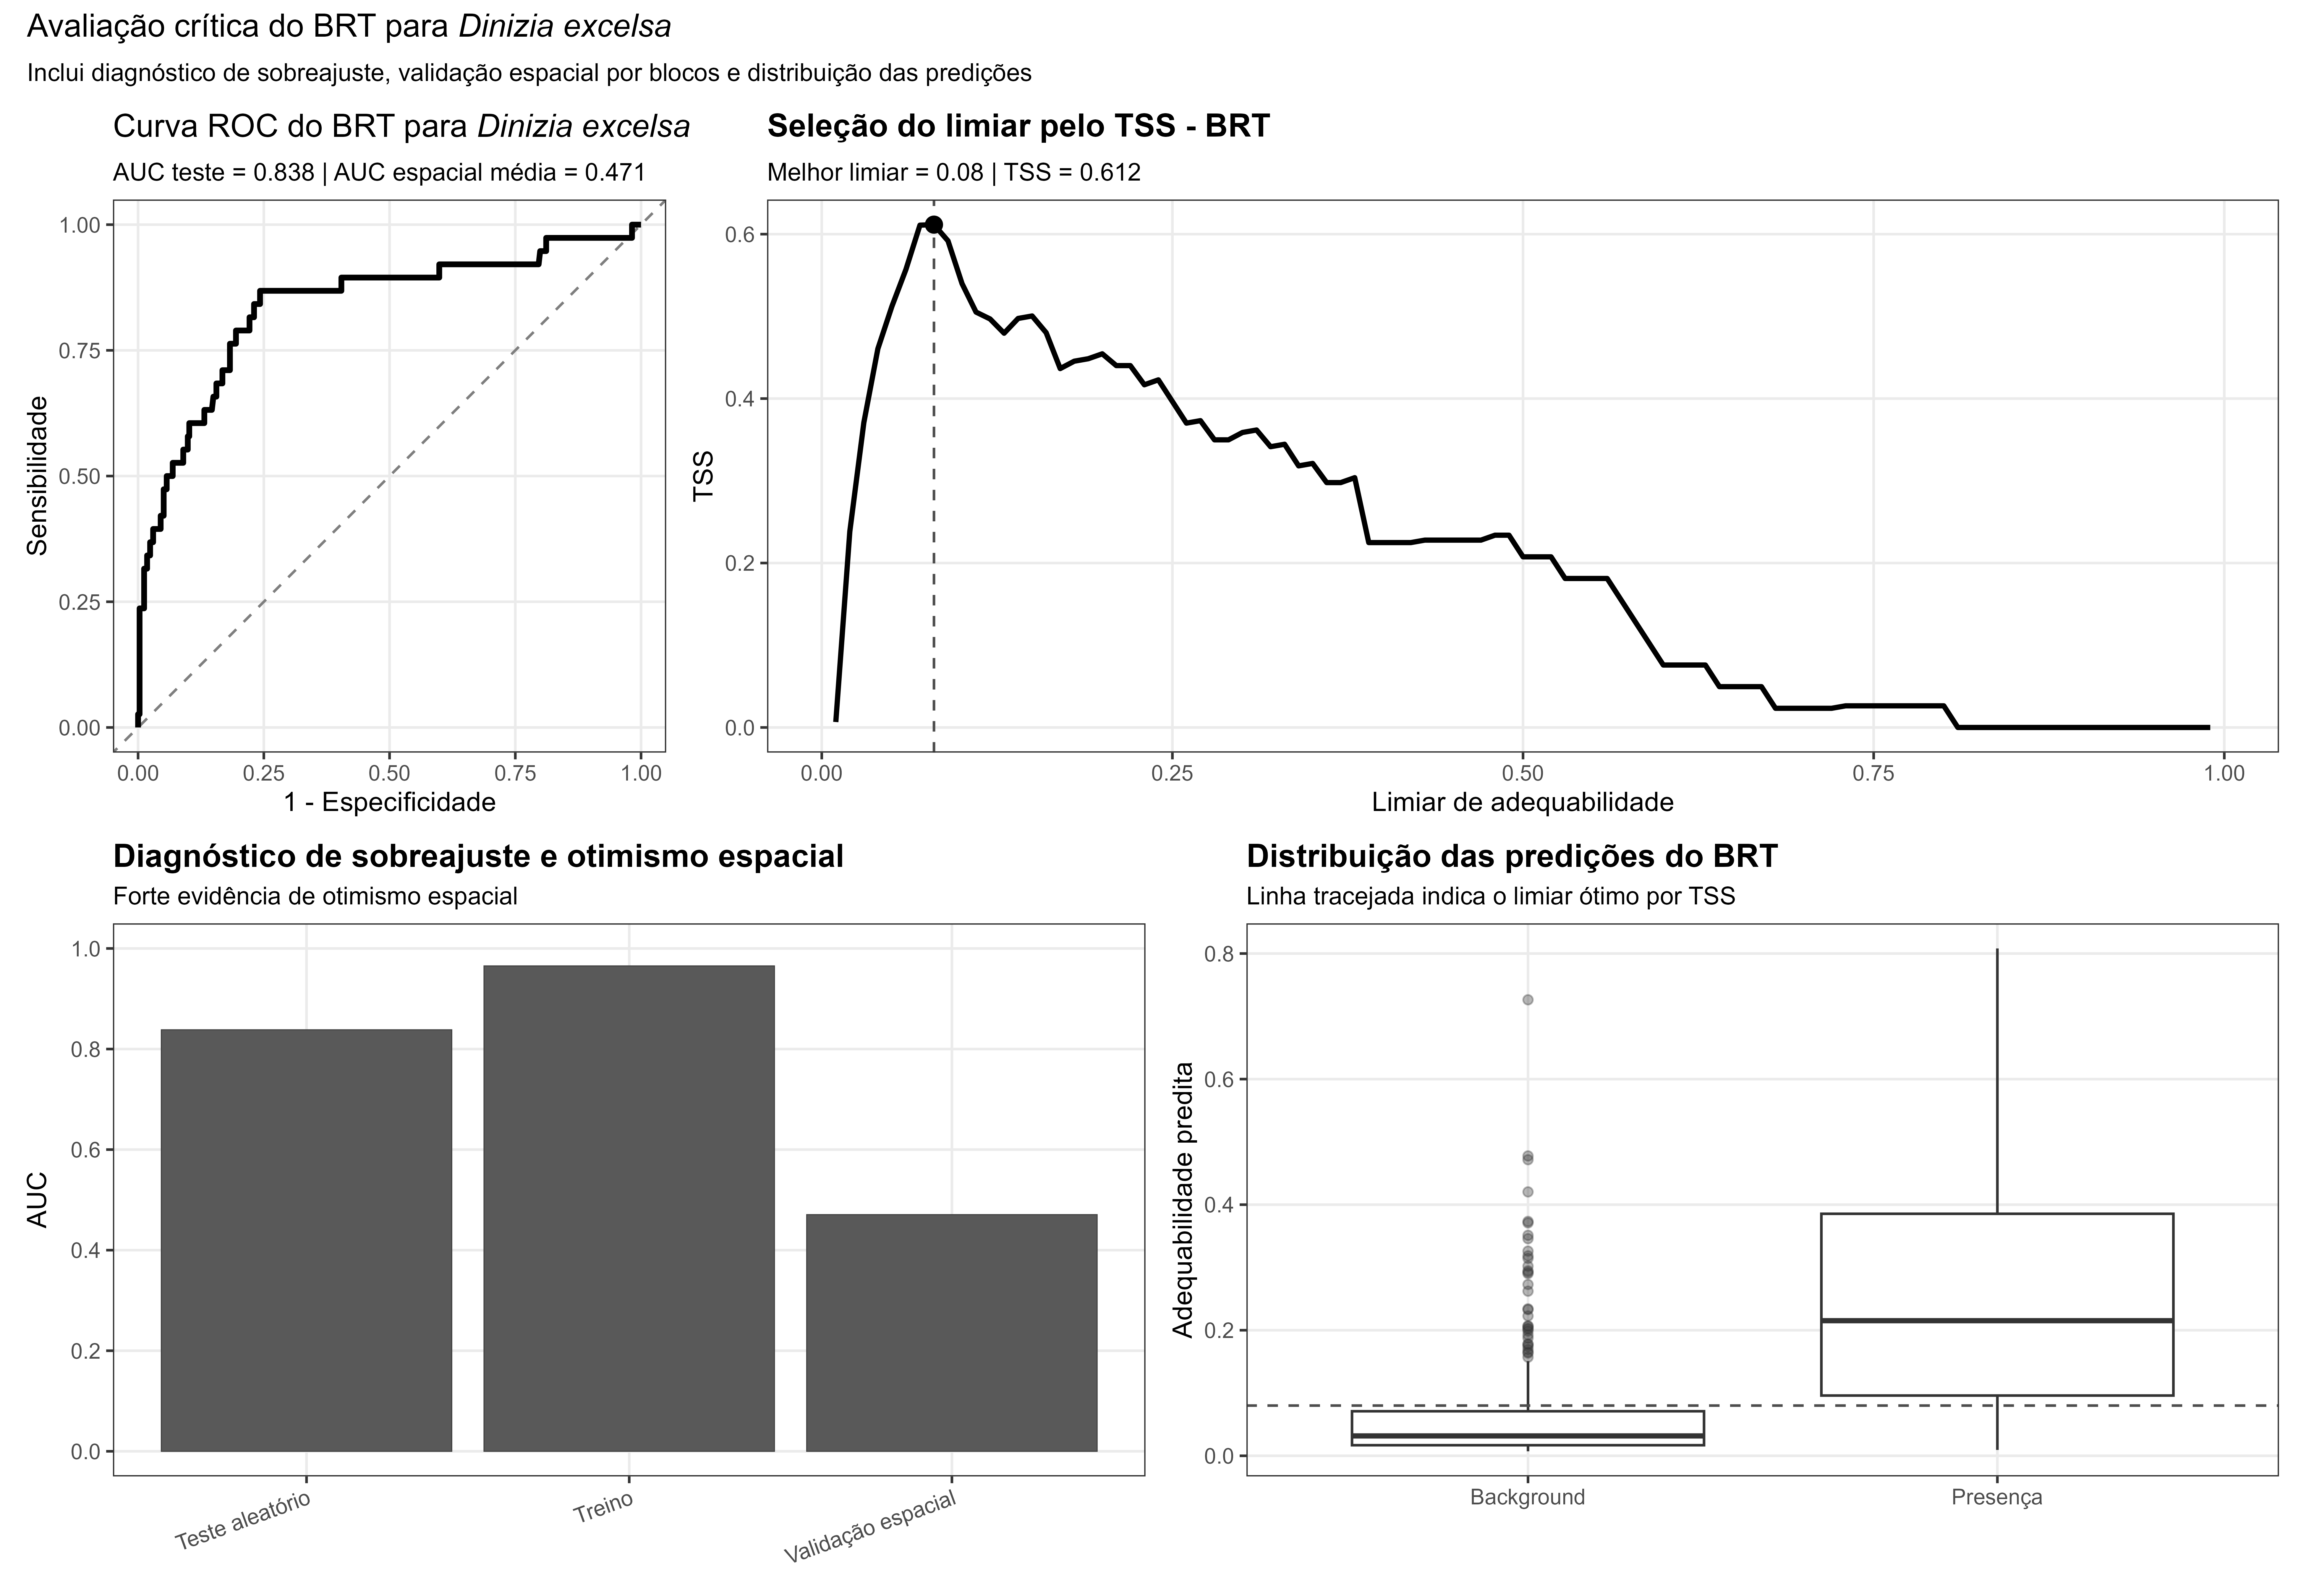
\includegraphics[width=0.78\textwidth]{figuras/unidade09/unidade09_avaliacao_brt_patchwork.png}
  \caption{ROC curve for the BRT evaluated on the test set.}
  \label{fig:unidade09_roc_brt}
\end{figure}

\begin{figure}[H]
  \centering
  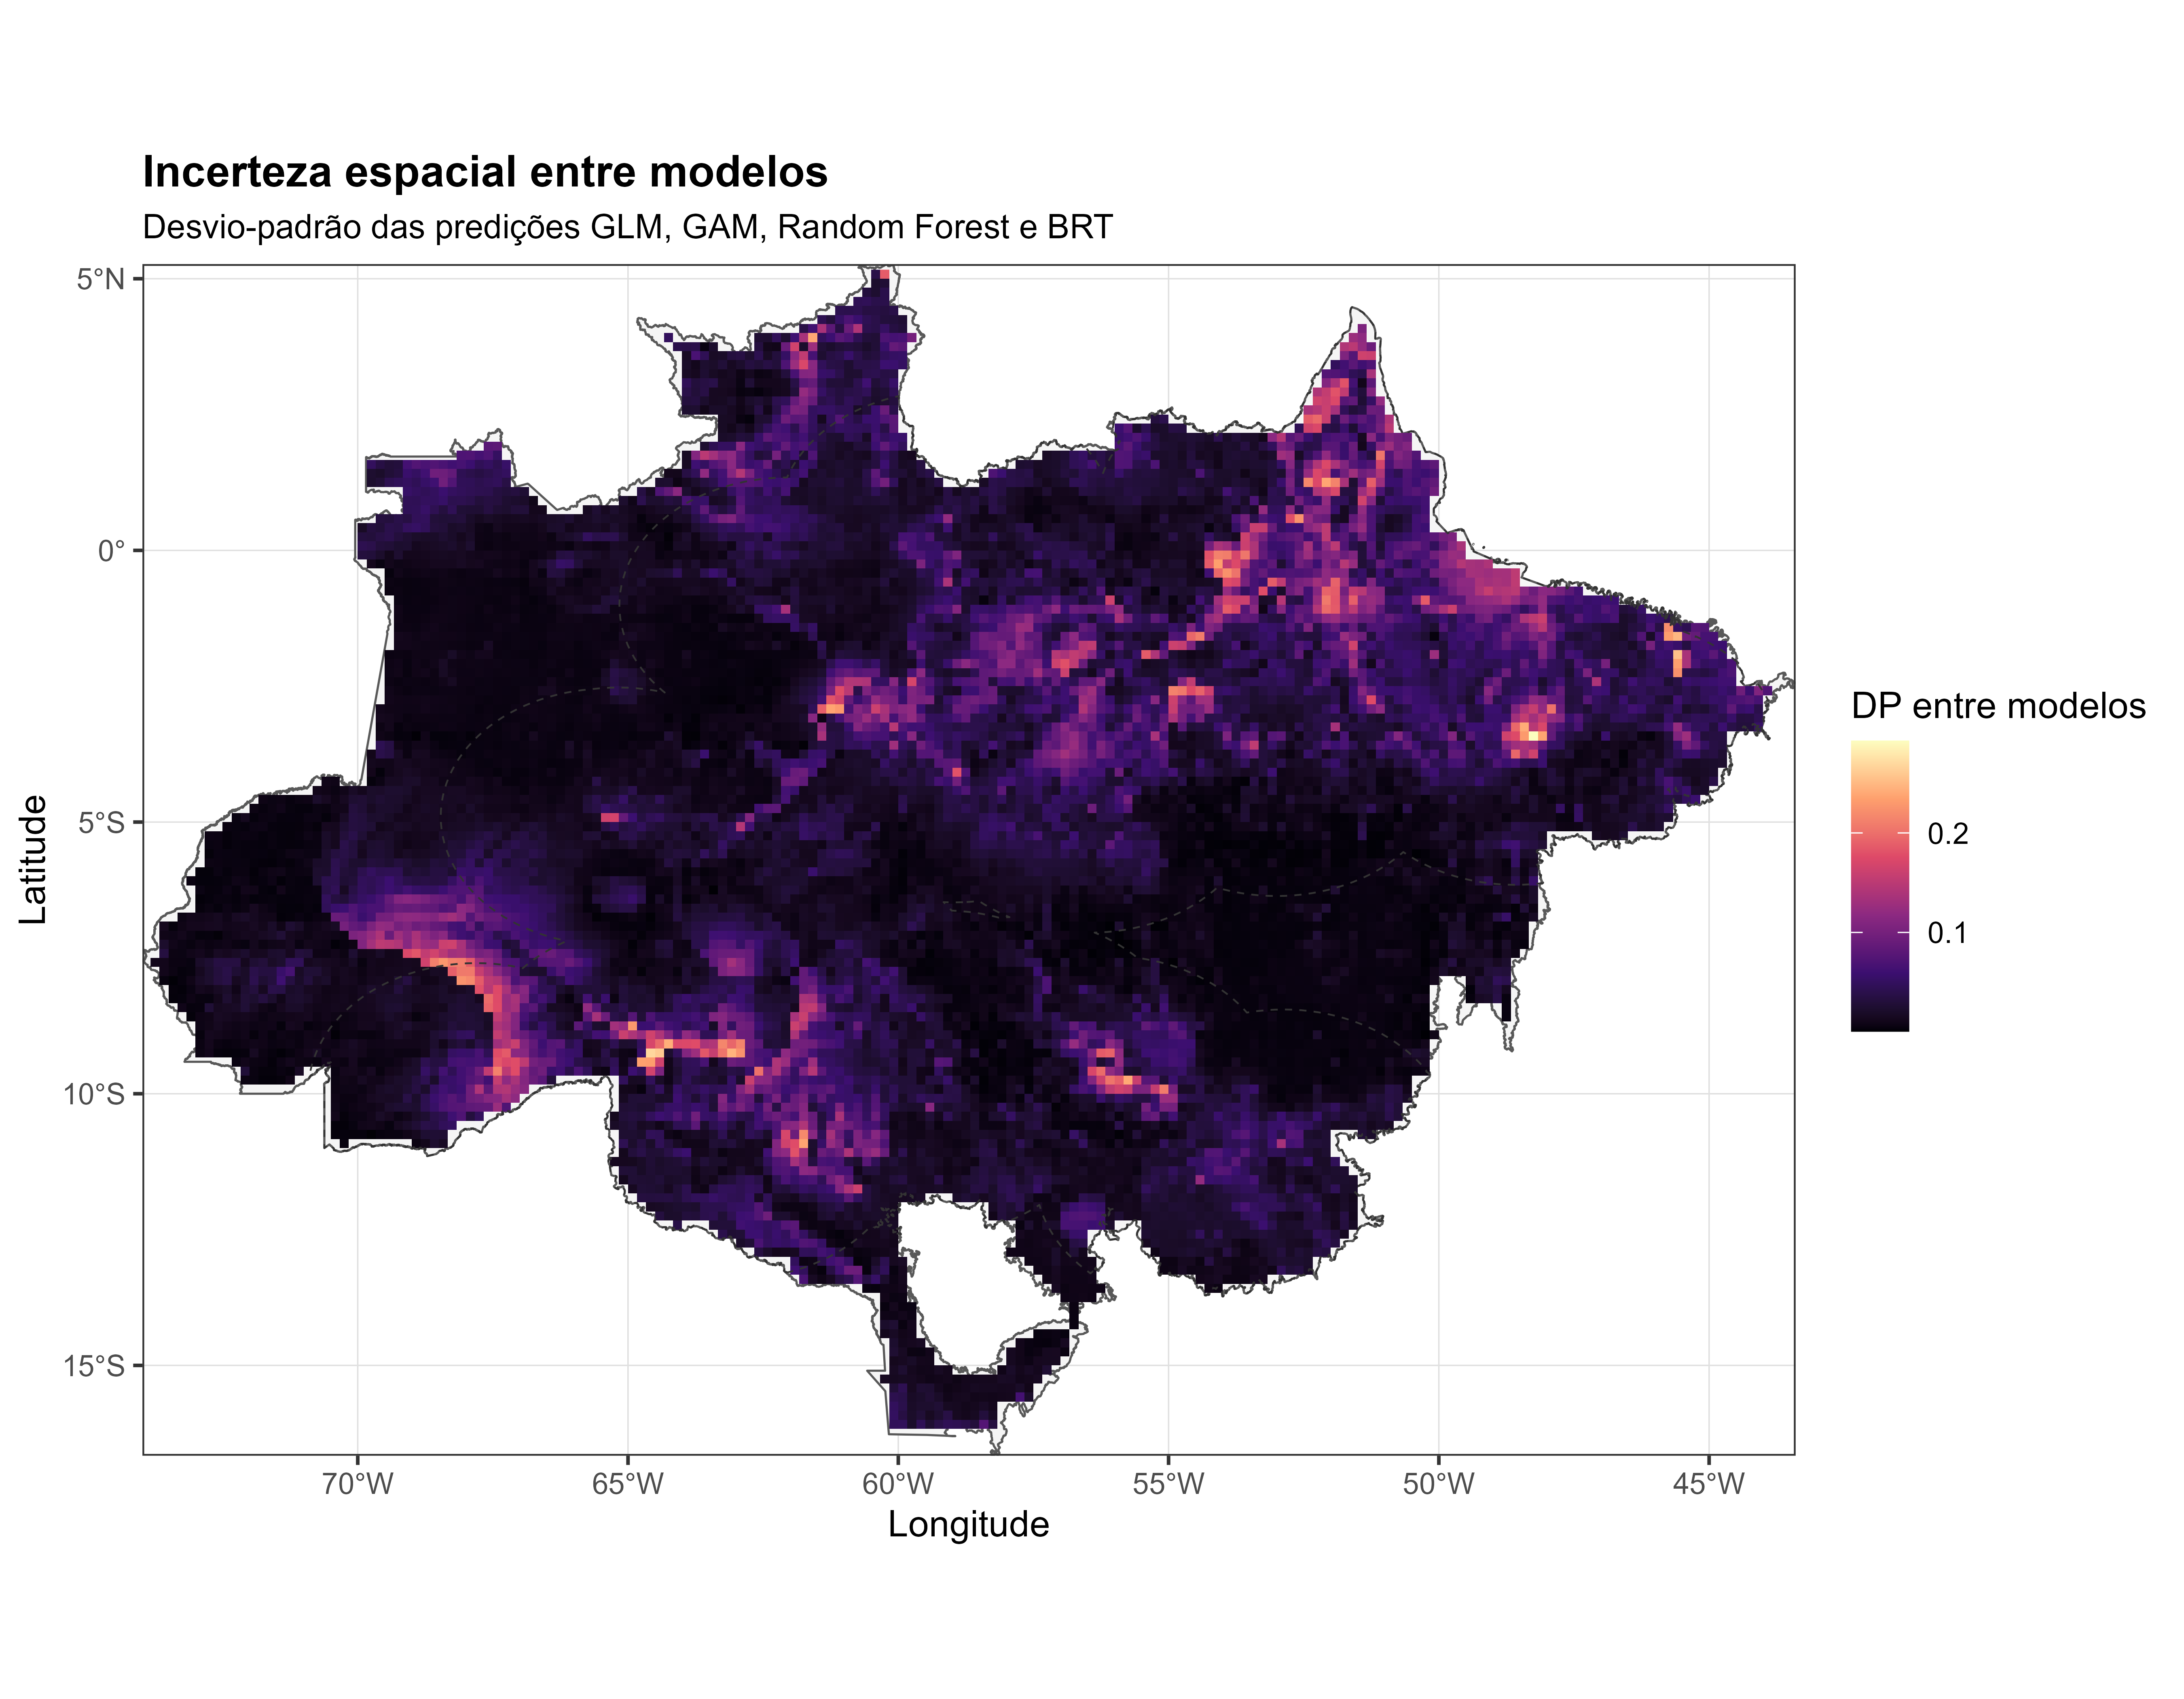
\includegraphics[width=0.78\textwidth]{figuras/unidade09/unidade09_incerteza_sd_glm_gam_rf_brt.png}
  \caption{Algorithmic disagreement for \textit{Dinizia excelsa}, calculated as the standard deviation among GLM, GAM, Random Forest, and BRT predictions. High values indicate weaker consensus among the fitted algorithms.}
  \label{fig:unidade09_incerteza_brt}
\end{figure}

\section{Current Suitability Map}
\rscriptfile{scripts/unidade09/05_predicao_espacial_brt.R}

\begin{figure}[H]
  \centering
  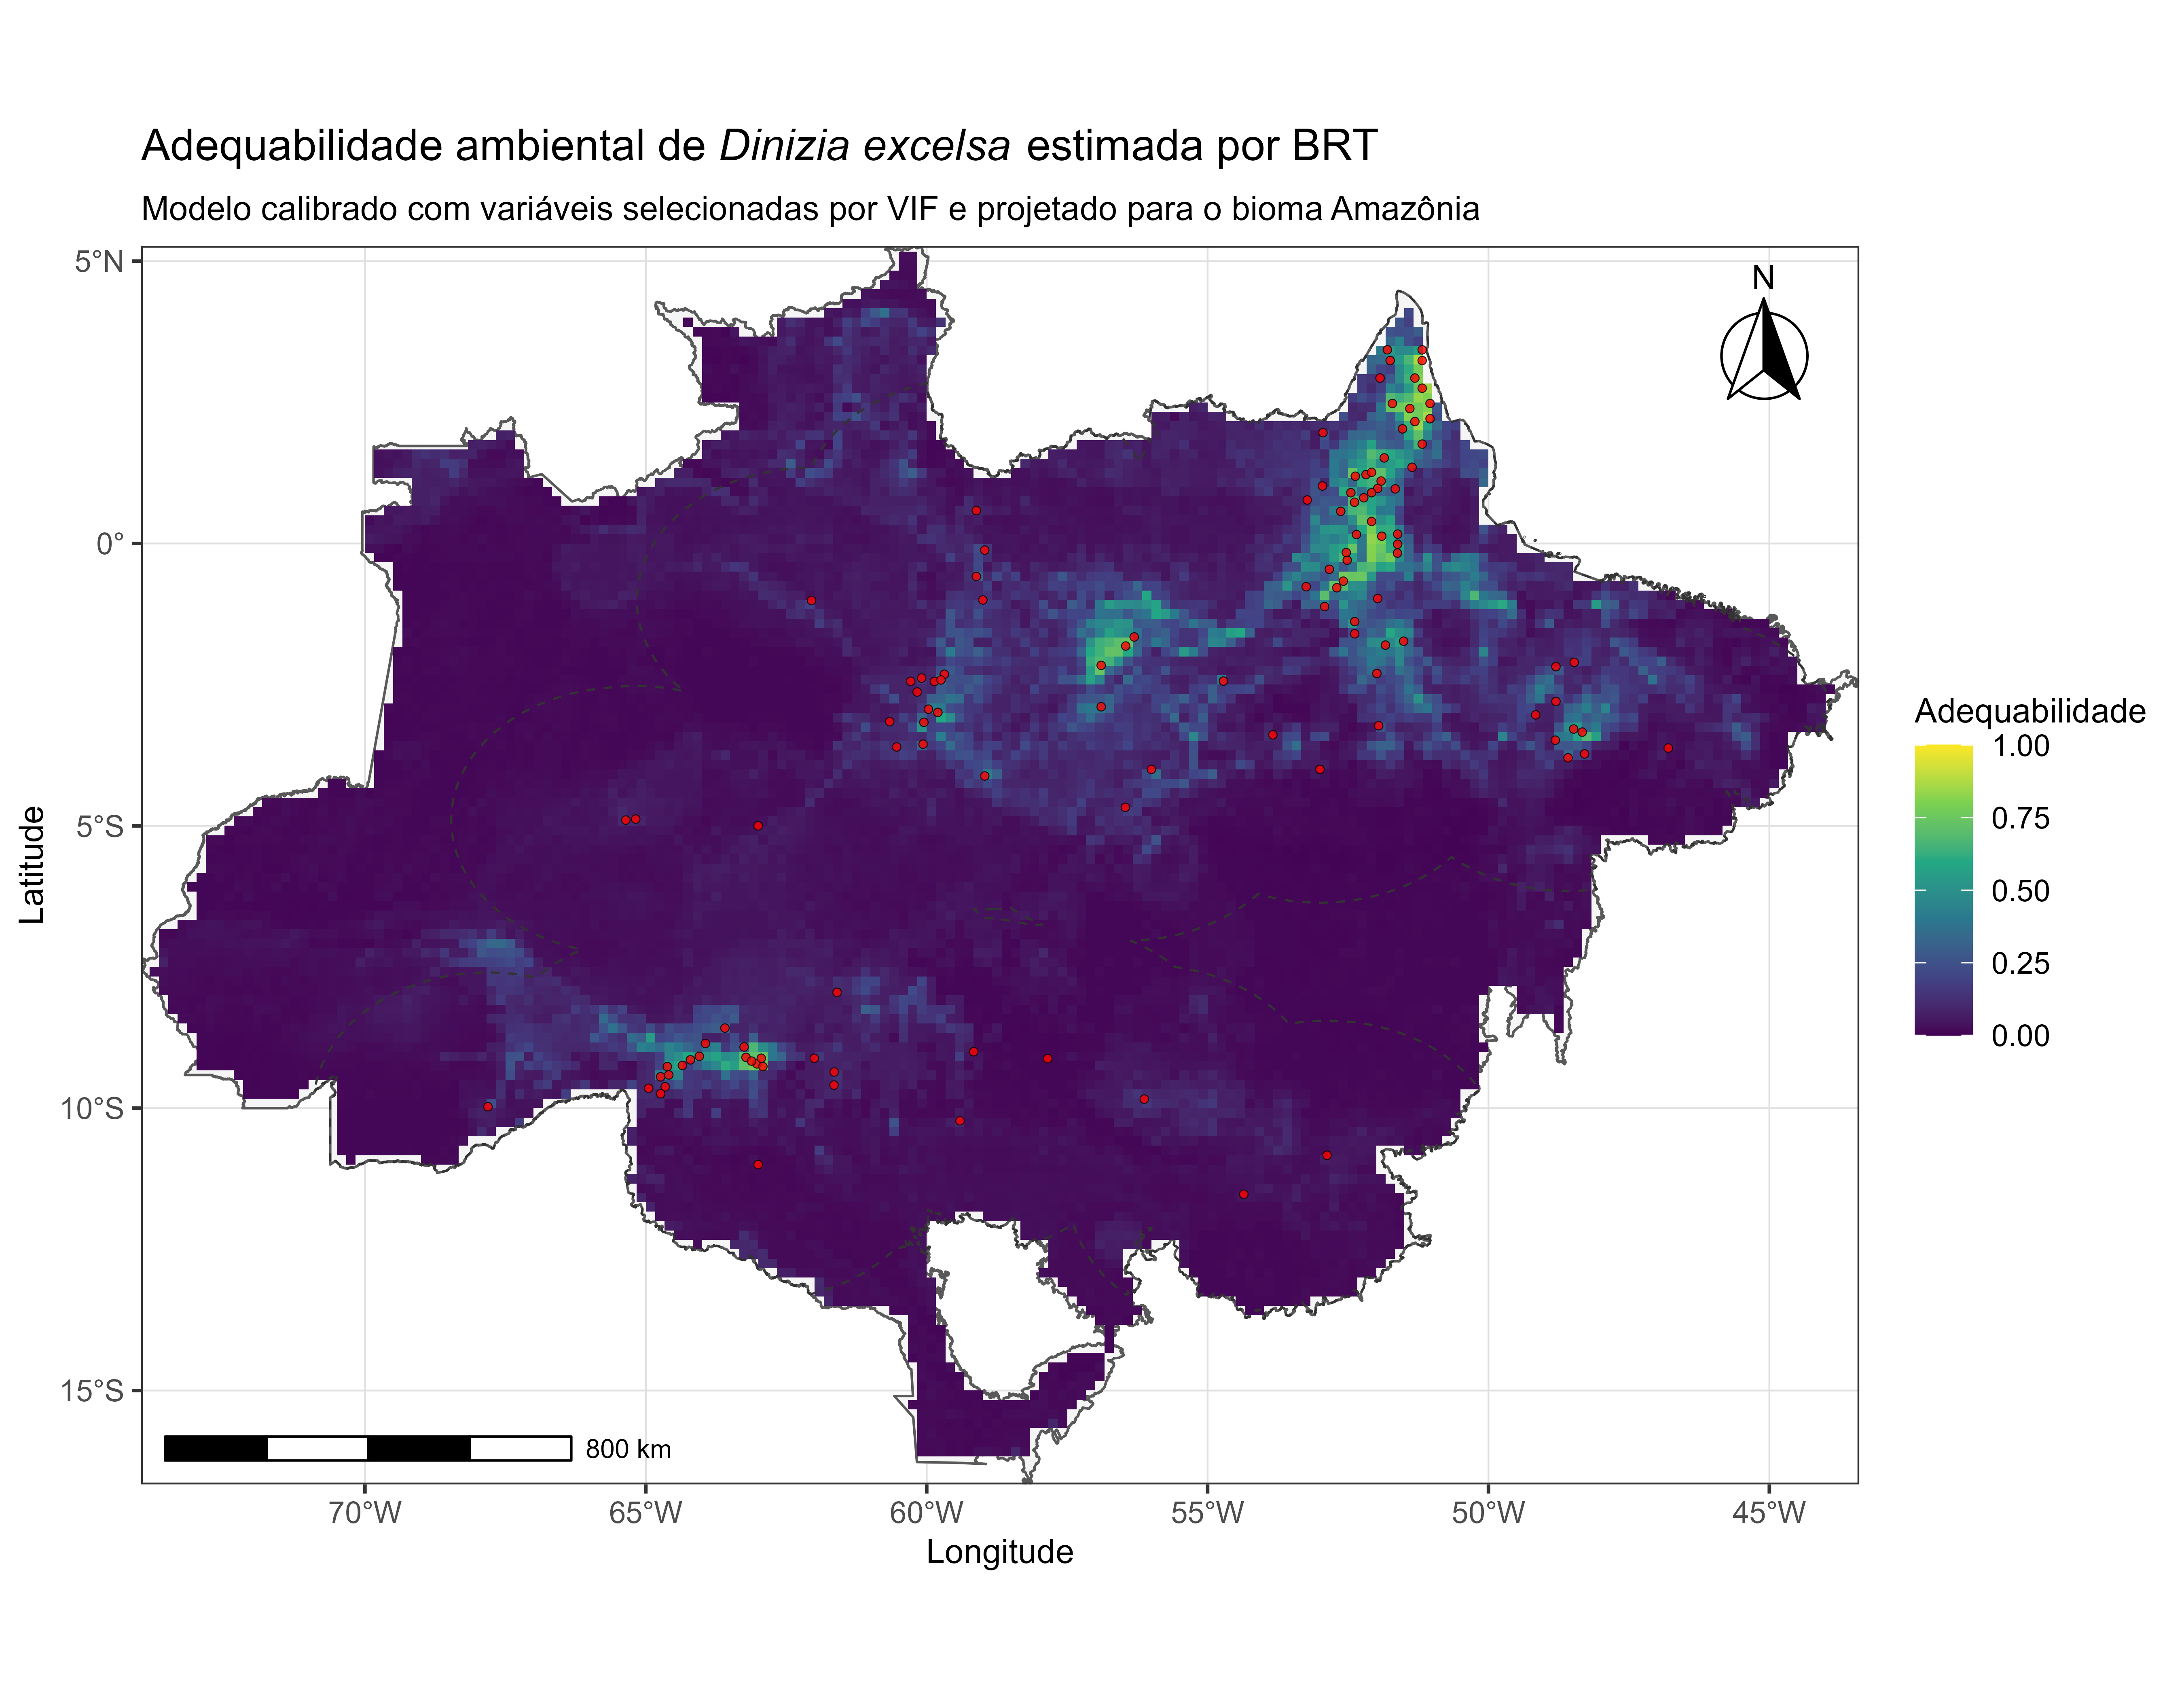
\includegraphics[width=0.88\textwidth]{figuras/unidade09/unidade09_adequabilidade_brt.png}
  \caption{Current suitability for \textit{Dinizia excelsa} estimated by BRT within the accessible area $M$.}
  \label{fig:unidade09_adequabilidade_brt}
\end{figure}

\section{Partial Response Curves}
\rscriptfile{scripts/unidade09/06_curvas_resposta_brt.R}

\begin{figure}[H]
  \centering
  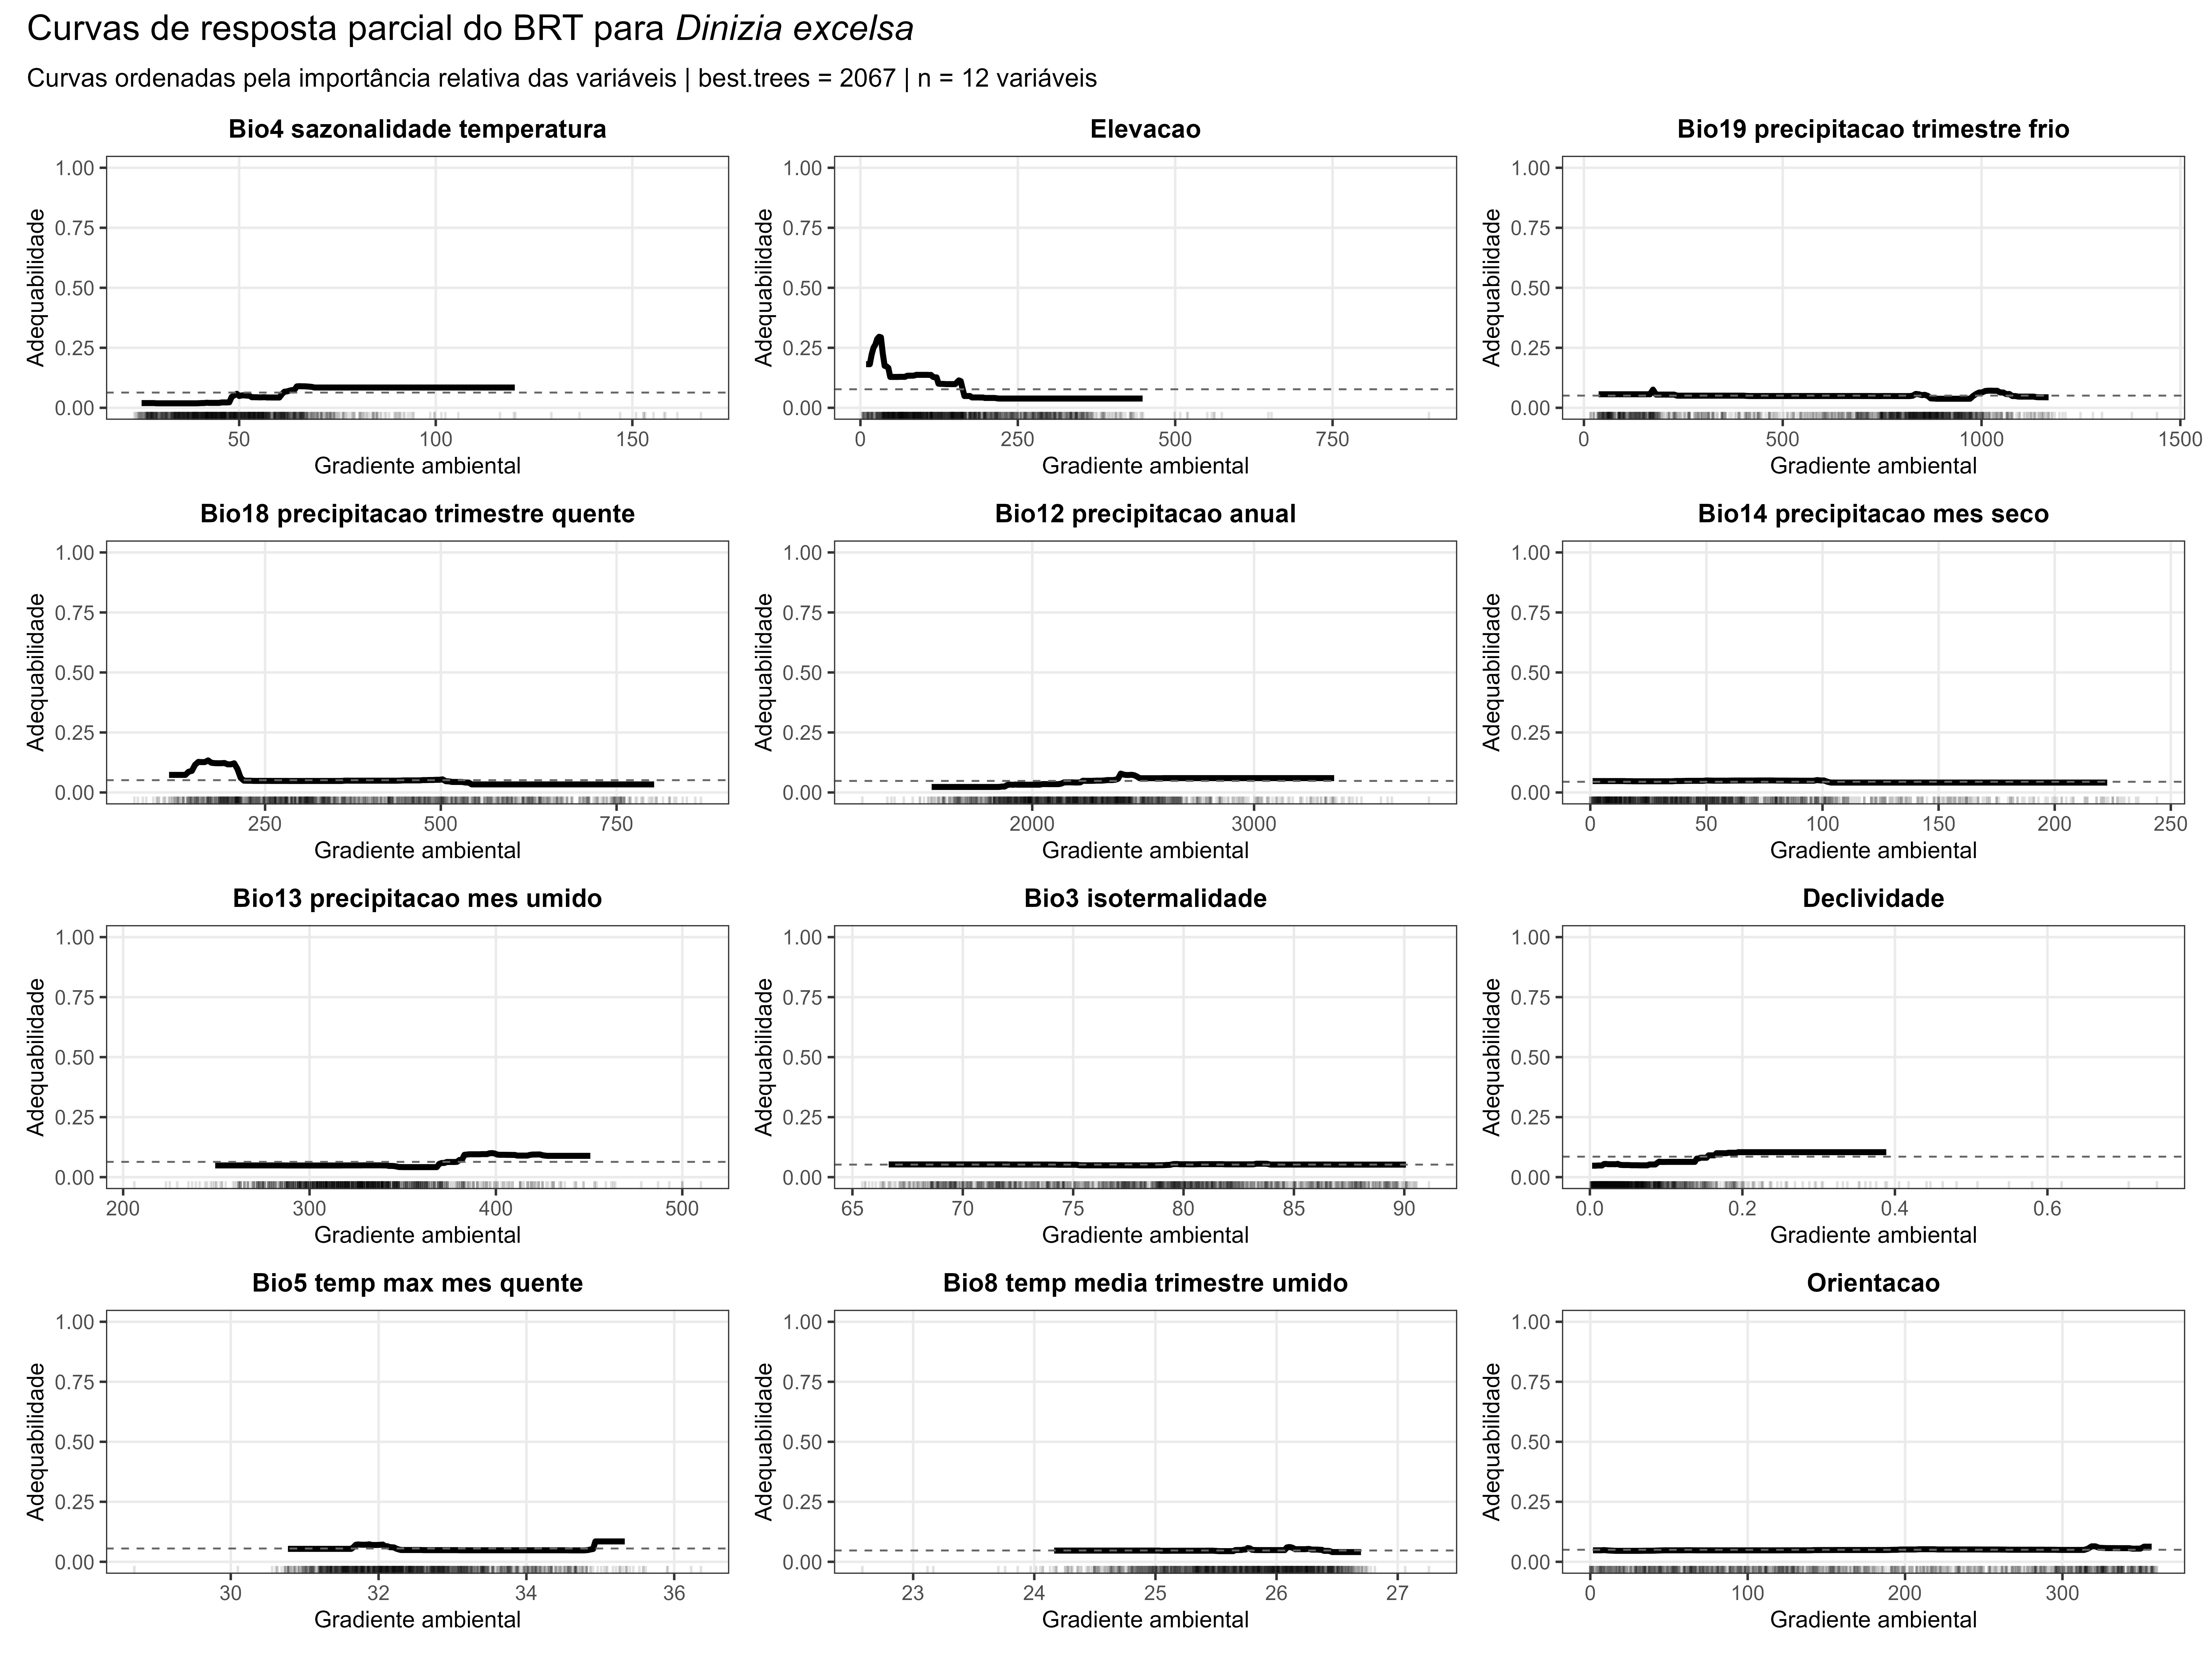
\includegraphics[width=0.96\textwidth]{figuras/unidade09/unidade09_curvas_resposta_brt.png}
  \caption{BRT partial response curves for the selected environmental predictors.}
  \label{fig:unidade09_curvas_resposta_brt}
\end{figure}

\section{Comparison with GLM, GAM, and Random Forest}
\rscriptfile{scripts/unidade09/07_comparar_modelos_brt.R}

\begin{figure}[H]
  \centering
  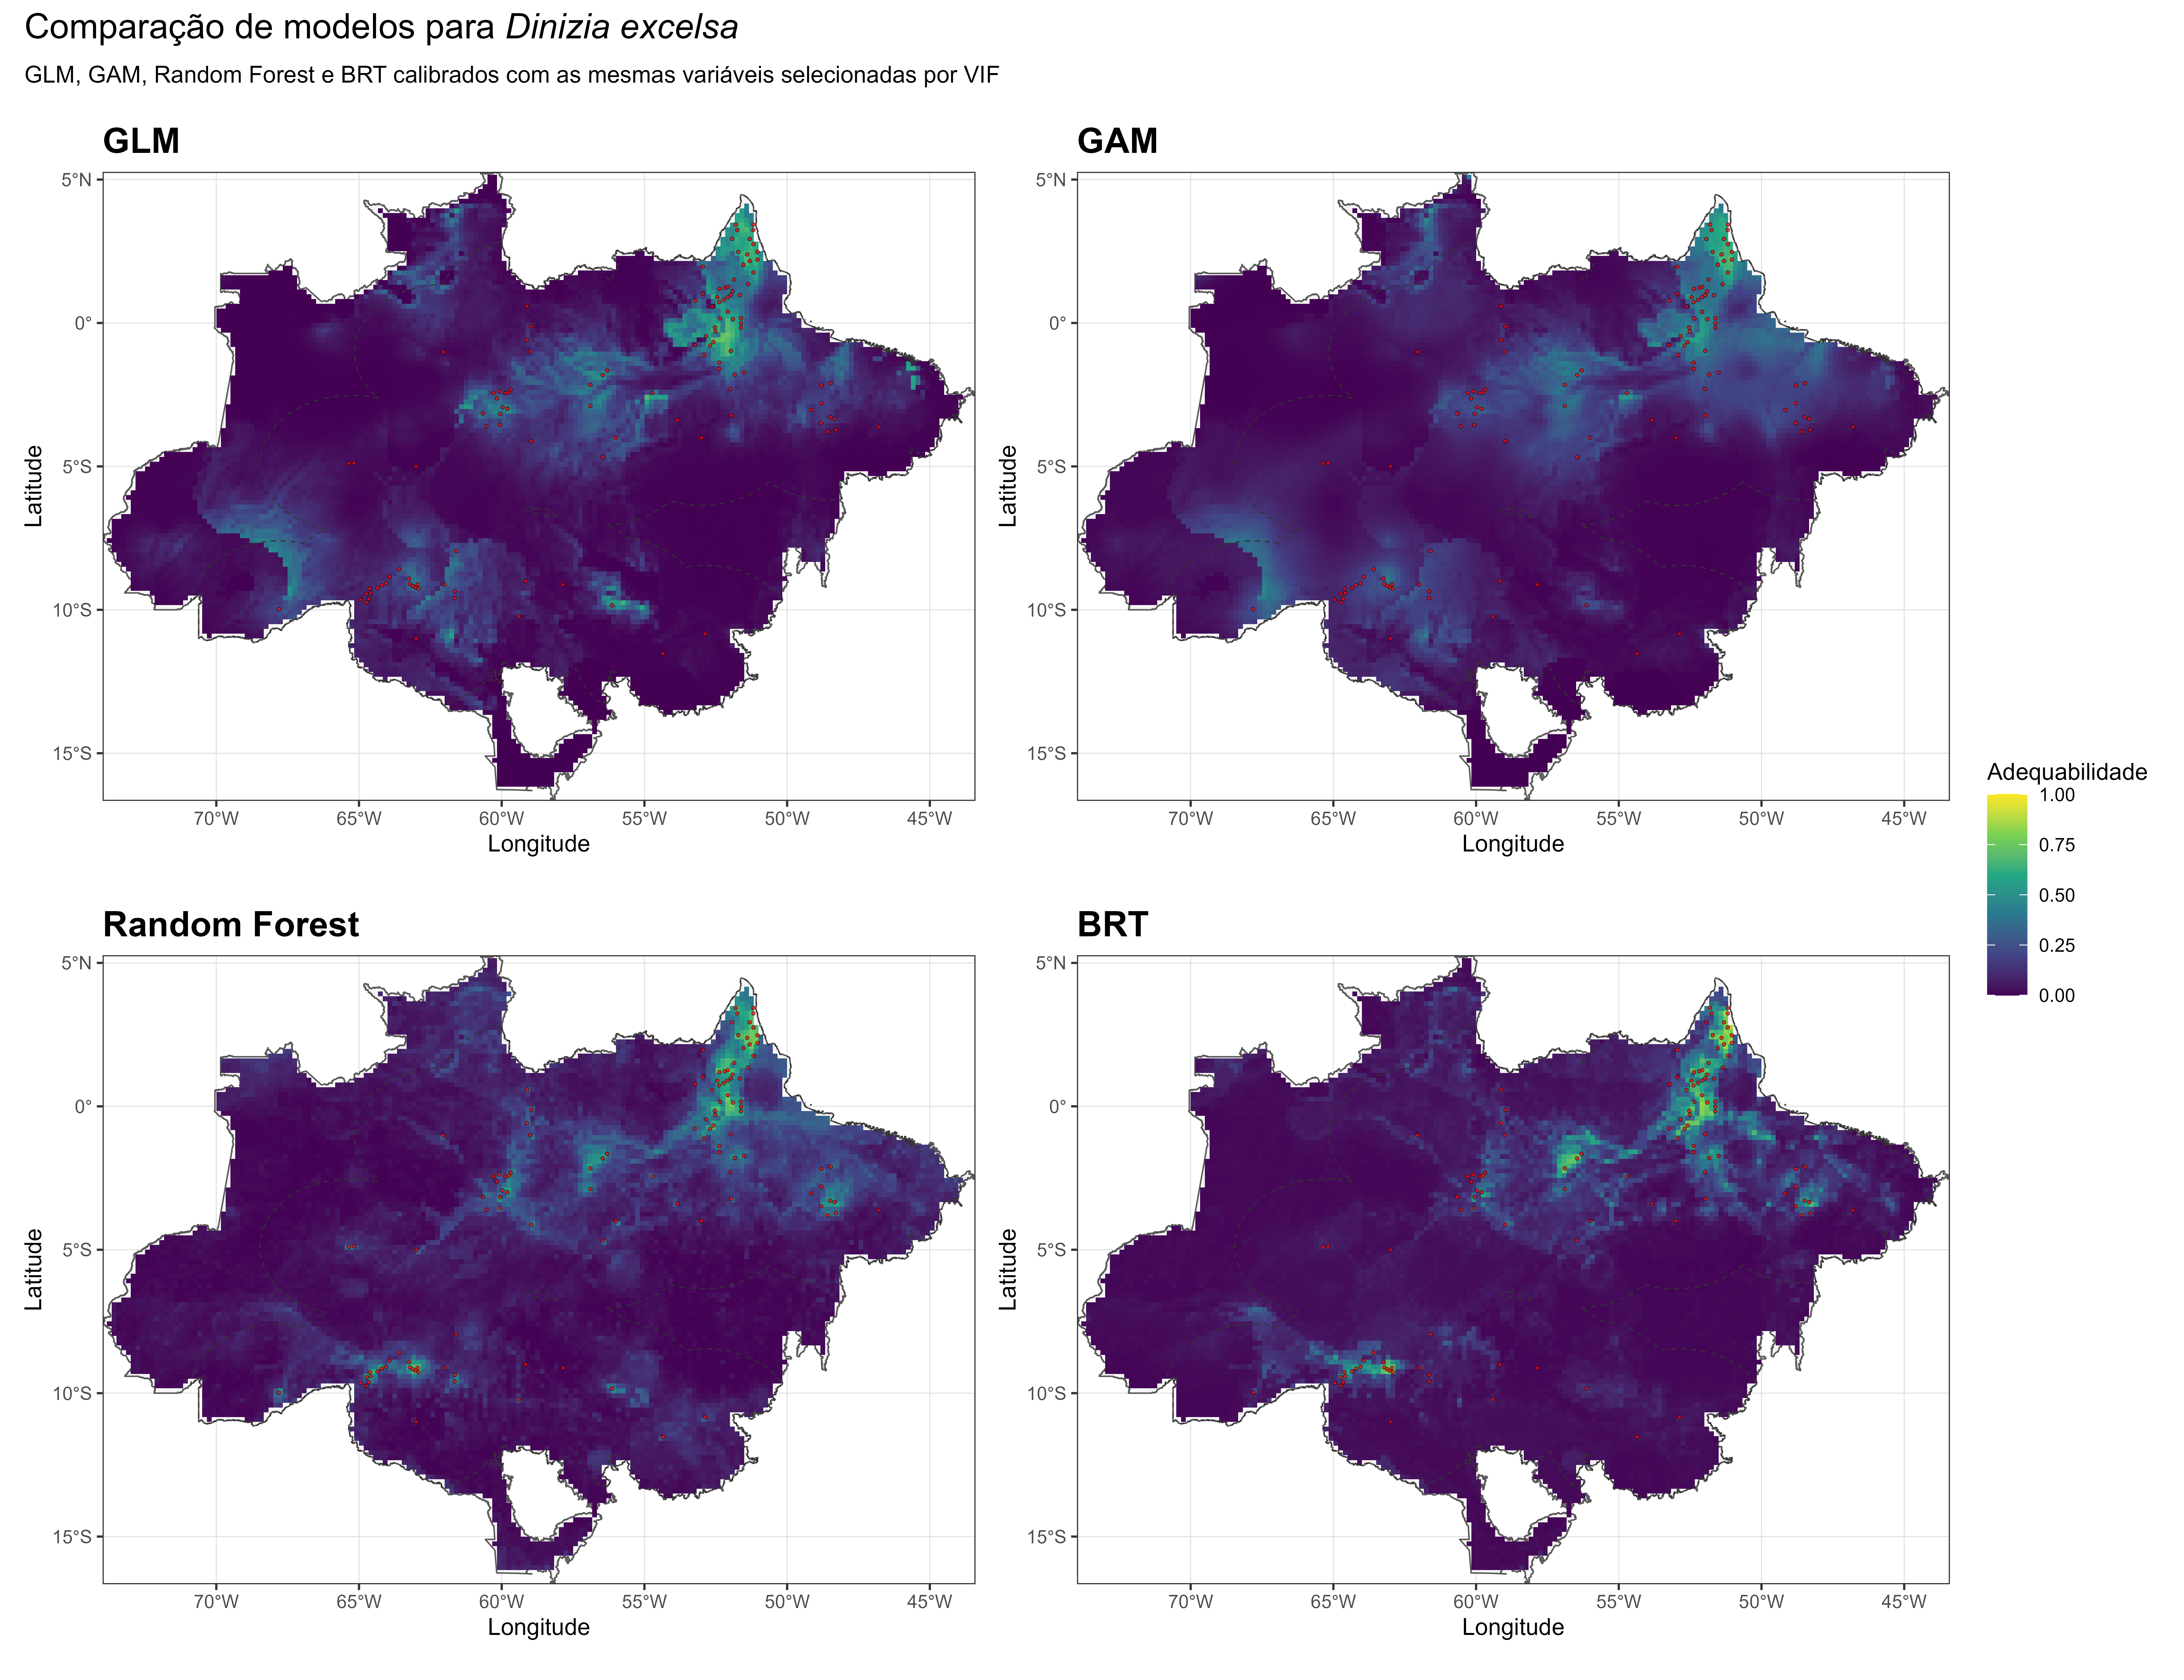
\includegraphics[width=0.96\textwidth]{figuras/unidade09/unidade09_comparacao_glm_gam_rf_brt.png}
  \caption{Comparison of suitability maps estimated by GLM, GAM, Random Forest, and BRT.}
  \label{fig:unidade09_comparacao_modelos}
\end{figure}

\section{Complete Pipeline}
\rscriptfile{scripts/unidade09/08_pipeline_brt.R}

\section{Chapter Summary}

BRT combines flexibility, interactions, and strong predictive performance, but
requires careful hyperparameter control and evaluation with independent data.

\begin{conceito}[title={\faBook\quad Key message}]
BRT can reveal complex environmental responses, but its credibility depends on
appropriate validation, overfitting control, and ecological interpretation.
\end{conceito}

\section{Review Exercises}
\begin{enumerate}
  \item Explain the difference between Random Forest and BRT.
  \item What does boosting mean?
  \item Why is \texttt{shrinkage} important?
  \item What is the role of \texttt{interaction.depth}?
  \item Why should cross-validation select the optimal number of trees?
  \item How is relative predictor importance interpreted in BRT?
  \item Why should partial response curves be evaluated critically?
\end{enumerate}
